\section{Фігури Ліссажу}
\textbf{Фігури Ліссажу} -- траекторії, які креслить точка, що здійснює 
гармонічні коливання у 2-х взаємно-перпендикулярних напрямках.

Отже, для їх побудови потрібні 2 параметричні рівняння: $x(t)$ та $y(t)$, які в загальному випадку не зводяться до залежності виду $y(x)$.
% ЩІТО? нам потрібні два сигнали, тому що в режимі Y(t)
% ми не можемо задавати змінну t, бо це, бляха, час. 
% Які параметричні залежності ти хочеш від генератора отримувати?
Оскільки генератор напряму не може видавати параметричних залежностей, \textit{лише з його допомогою} фігури Ліссажу побудувати не вдасться.

Для досягнення мети ми використовували чотирьохполюсник, підключений як на рисунку нижче. \\
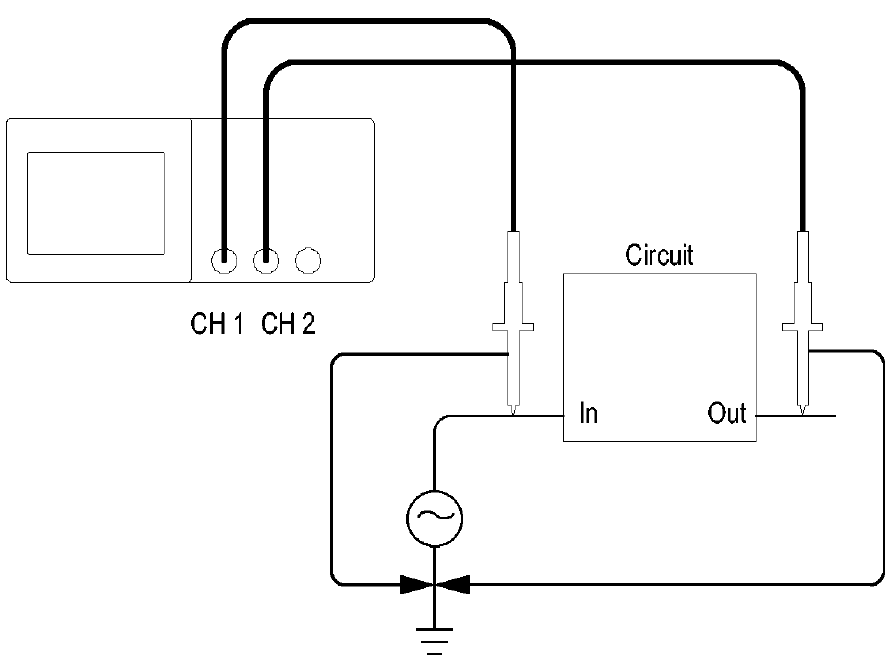
\includegraphics[width=\textwidth, keepaspectratio]{1-lab/res/4pole.png}

В нашому осцилографі функція <<\textbf{МЕНЮ К2}>> була відсутня. Тому ми послідовно натискали на ньому наступні кнопки:
\begin{enumerate}
    \item \textbf{МЕНЮ К1}.
    \item \textbf{АВТОУСТ}.
    \item \textbf{ВОЛЬТ/ДЕЛ} (вирівнювали амплітуди сигналів).
    \item \textbf{ЭКРАН}.
    \item \textbf{ФОРМАТ} $\rightarrow$ \textbf{XY}. 
    \item \textbf{ВОЛЬТ/ДЕЛ}, \textbf{ВЕРТИК. ПОЛОЖЕНИЕ} (встановлювали зображення, зручне для роботи).
    \item \textbf{Presist} $\rightarrow$ \textbf{Infinite}.
    \item \textbf{Adjust Contrast} (змінювали контрастність зображення).
    
\end{enumerate}

В результаті були отримані такі фігури Лісажу:\\ 
\\
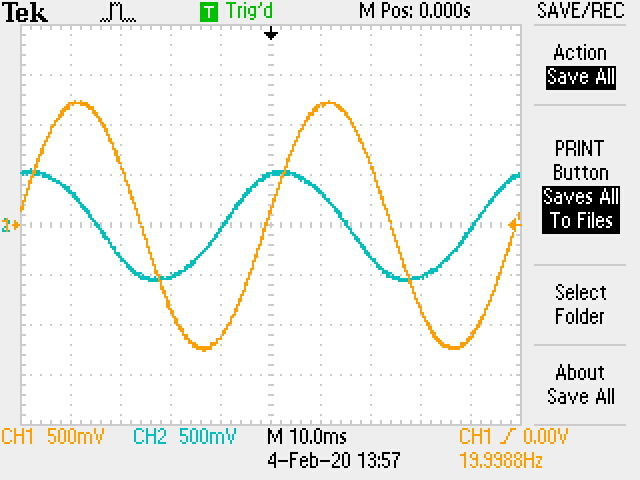
\includegraphics[width=\textwidth/2]{1-lab/res/3a.JPG}
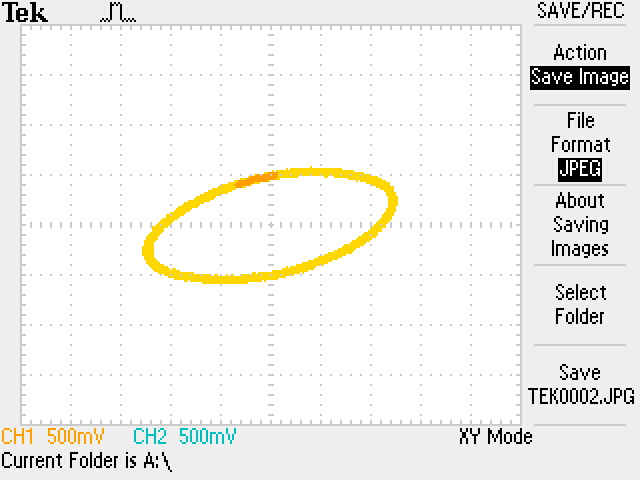
\includegraphics[width=\textwidth/2]{1-lab/res/3b.JPG}\\
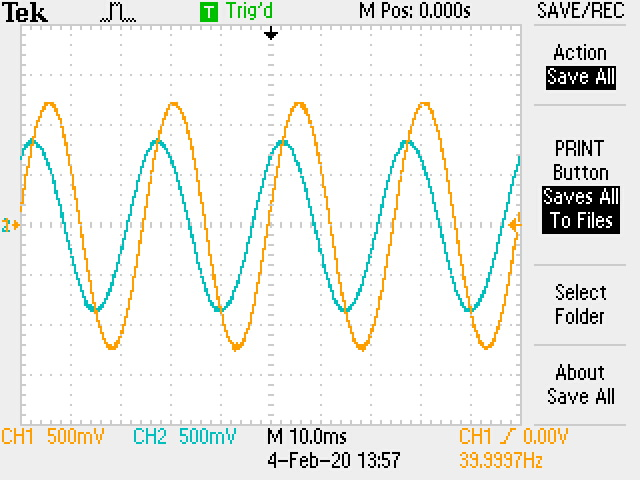
\includegraphics[width=\textwidth/2]{1-lab/res/4a.JPG}
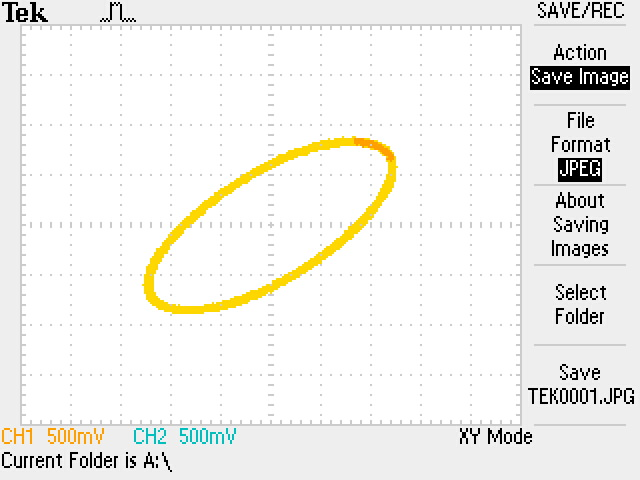
\includegraphics[width=\textwidth/2]{1-lab/res/4b.JPG}\\
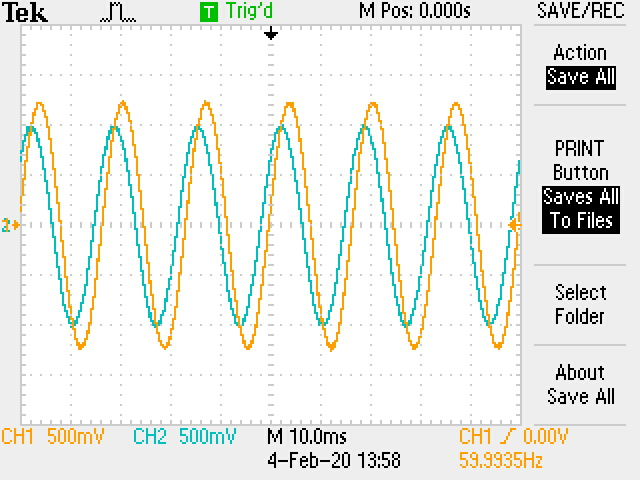
\includegraphics[width=\textwidth/2]{1-lab/res/5a.JPG}
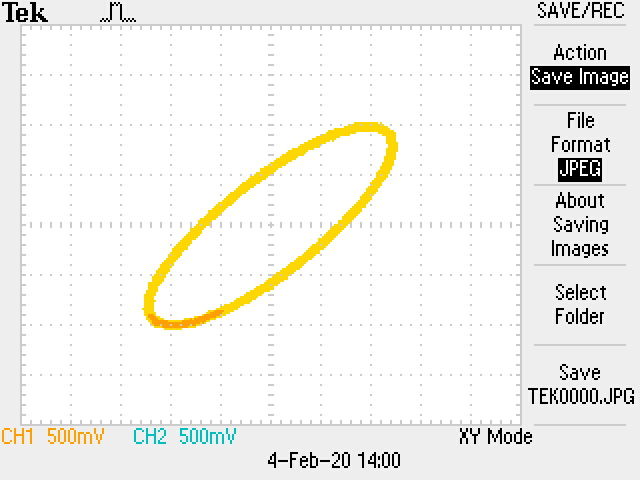
\includegraphics[width=\textwidth/2]{1-lab/res/5b.JPG}

